\documentclass{article}
\usepackage{graphicx}
\usepackage{amsmath}
\usepackage[parfill]{parskip}
\usepackage{hyperref}
\graphicspath{ {./figures/} }

\title{COMP.SEC.220 Security Protocol\footnote{github --- \url{https://github.com/ancuongnguyen07/SecurityProtocol}}}
\author{Cuong Nguyen --- LAB 7}
\date{05/10/2022}

\begin{document}
    
\maketitle

\begin{figure}[hpt]
    \centering
    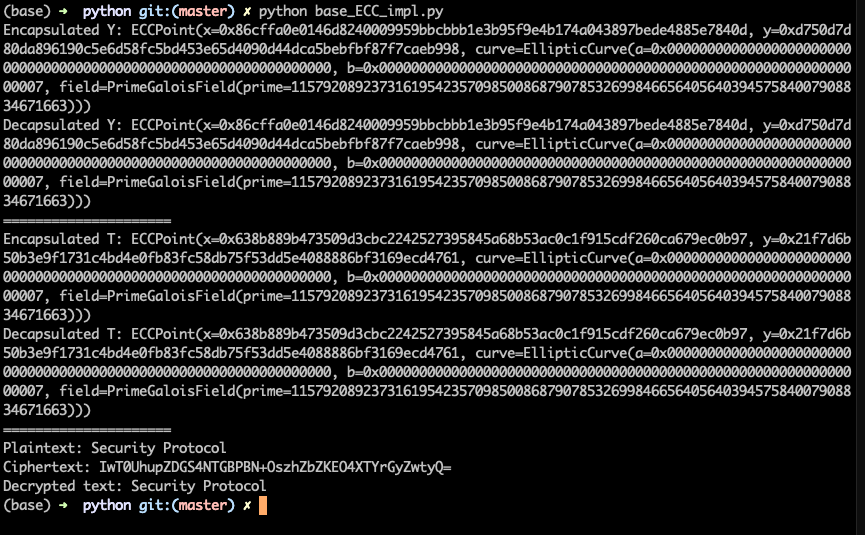
\includegraphics[height=\textheight,width=\textwidth,keepaspectratio
                    ]{sucessful_run.png}
    \caption{A successful run of the ECC implementation.}
\end{figure}

\emph{The encapsulated Y} (step 2) equals \emph{the decapsulated Y} (step 3).
The same observation also apply to the \emph{T} values. Source code:
\url{https://github.com/ancuongnguyen07/SecurityProtocol/blob/master/lab7/python/base_ECC_impl.py}

\end{document}